\section{Web Interface}
\index{Web Interface}

The built in web interface provides a set of pages that control and monitor the WebBrick, these are described here. 
Generally on the web interface if an item is clickable it will be highlighted and change colour when 
the mouse cursor runs over it. The highlight will only be active for most areas when the UI is logged in.

\subsection{Logged in}

	The default configuration of a WebBrick has no password for the \em{control} web pages.  You'll
	need a password for the configuration and installer pages.  A password can be set for 
        the \em{control} pages in which case the controls on the home page are hidden.  The default passwords
        are 'password' for the configuration pages and 'installer' for all areas.

\subsection{All Pages}
All the web pages have a banner section that contains the WebBrick logo, the node name and number, 
the current time, current operational state (with an indication on whether it is logged in). 
This banner may go Red if the last command received by the PIC chip was invalid.

Under this section are a set of links that select other web pages.  Some of these links are hidden
until the WebBrick validates them, i.e 'Configure Server' is only visible once logged in.

\subsection{Triggers}
The various inputs channels can generate triggers events that can then cause action on the outputs and/or a network
events to be sent. The configuration details for a trigger include a action a target channel  and additional action
dependant parameters.

\subsection{Home}
The home page or landing page shows the current state of the outputs and has a set of controls that can
be clicked to make changes to the outputs. The controls will be hideen if the level 1 password has been
set and you are not curently logged in.

\begin{figure}[H]
\centering
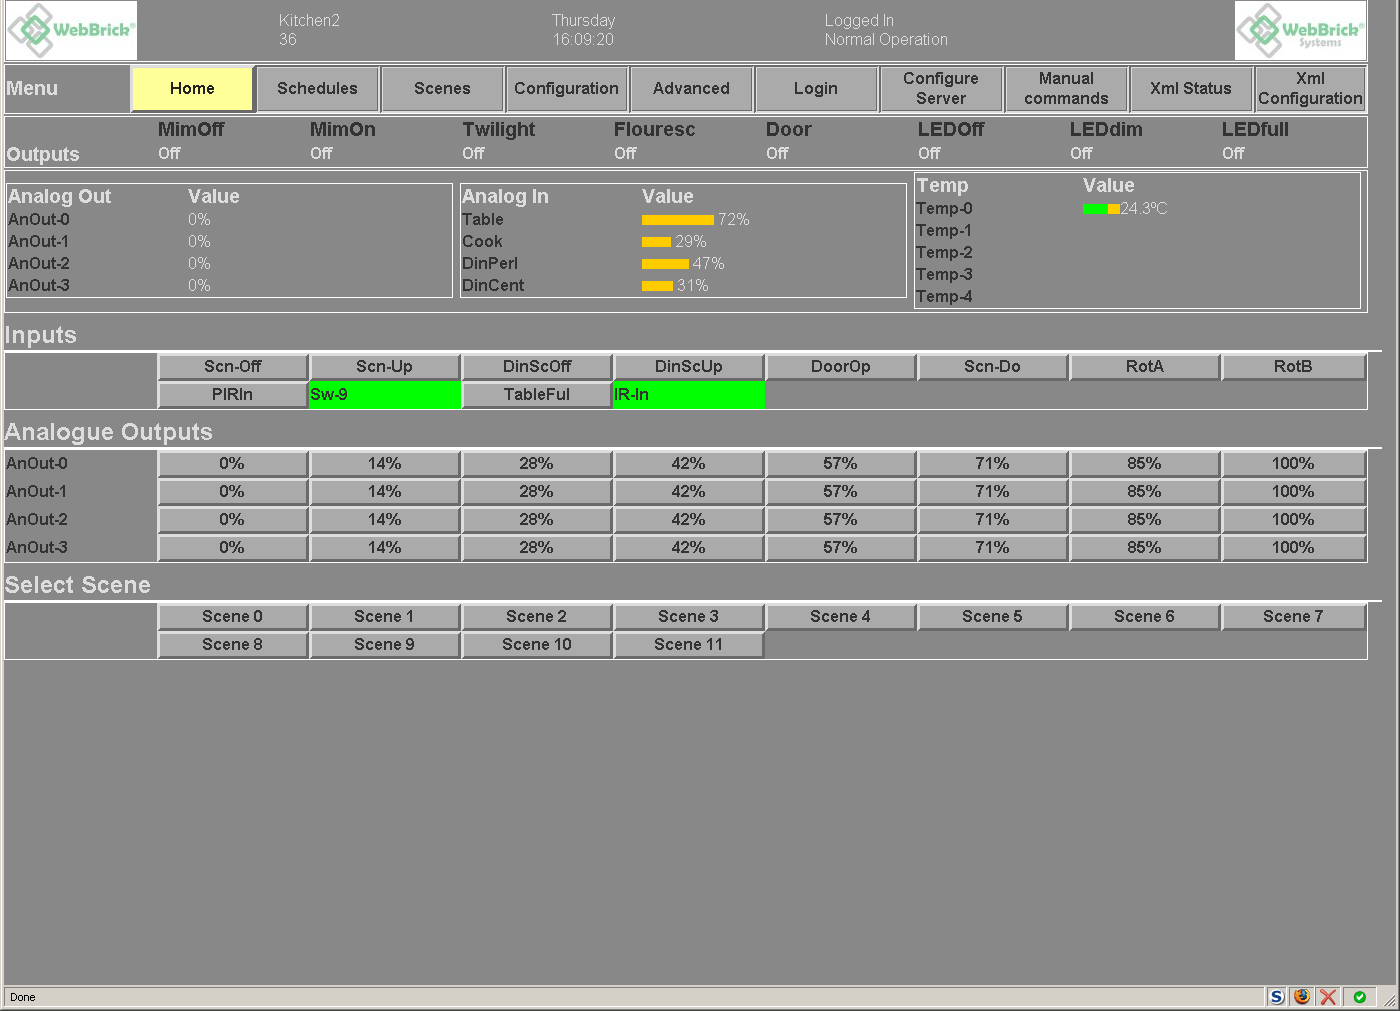
\includegraphics[width=0.8\textwidth]{Images/home.png}
\caption{WebBrick Standard Home Page}
\end{figure}


\begin{tabular}{l|p{12cm}}
Section&Description\\
\hline
1&The first section shows the state of the Digital Outputs, 
note that you will have to refresh the page for the current status.\\

2&The second section shows the state of the analogue inputs, outputs and temperature sensors.\\

3&The Digital Input trigger buttons are named as per their configuration.  Note that Digital inputs that 
have no action are treated as Monitors only and are not displayed as buttons.
Pressing these  buttons creates an event as if the physical button had been
operated.  This is useful for both remote control and confirming that a button does as you intended.\\

4&The Analogue table gives 8 buttons for each analogue output channel to set the Analogue outputs to any one of the 8 SetPoints.
The buttons are labelled with the value of the setpoint.\\

5&Finally there are buttons to set a specific scene.\\
\end{tabular}

\subsection{Schedules}

\begin{figure}[H]
\centering
\includegraphics[width=0.8\textwidth]{Images/schedules.png}
\caption{WebBrick Schedules Page}
\end{figure}

This page shows the current scheduled triggers and if logged in you can click on an entry to configure a scheduled event.
The configuration for a schedule entry consists of the days on which it is to happen and the time at which it should happen. 
When the correct day and time occurs the targetted channel will be actioned, this could be a single output channel or one of 
the scenes.

\begin{figure}[H]
\centering
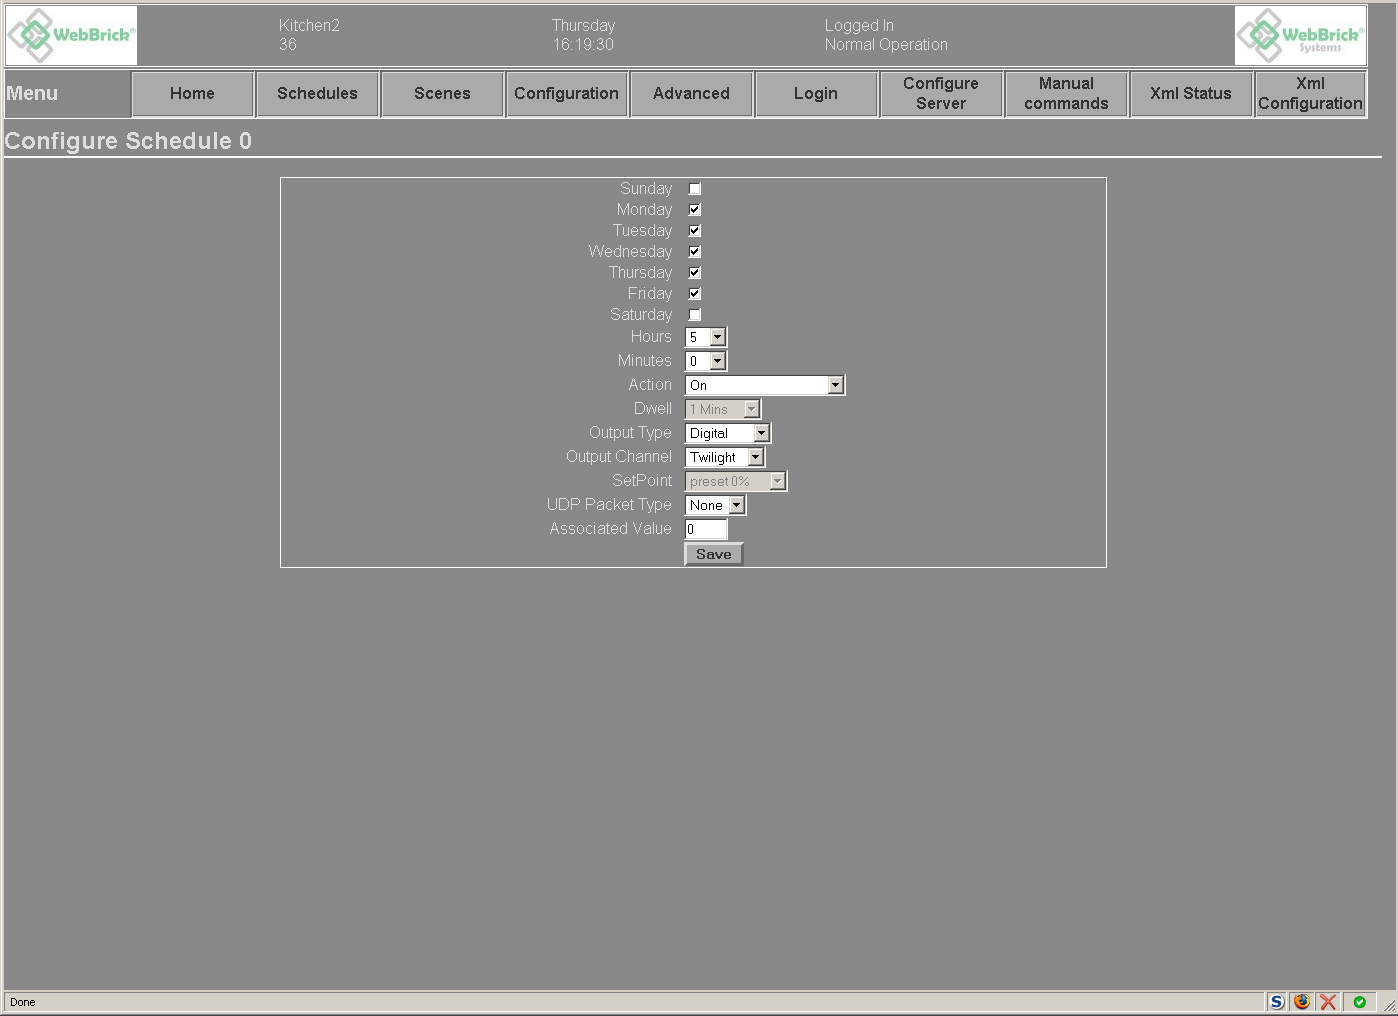
\includegraphics[width=0.8\textwidth]{Images/schedule.png}
\caption{WebBrick Schedule configuration Page}
\end{figure}

\subsection{Scenes}
\index{Scenes}
\begin{figure}[H]
\centering
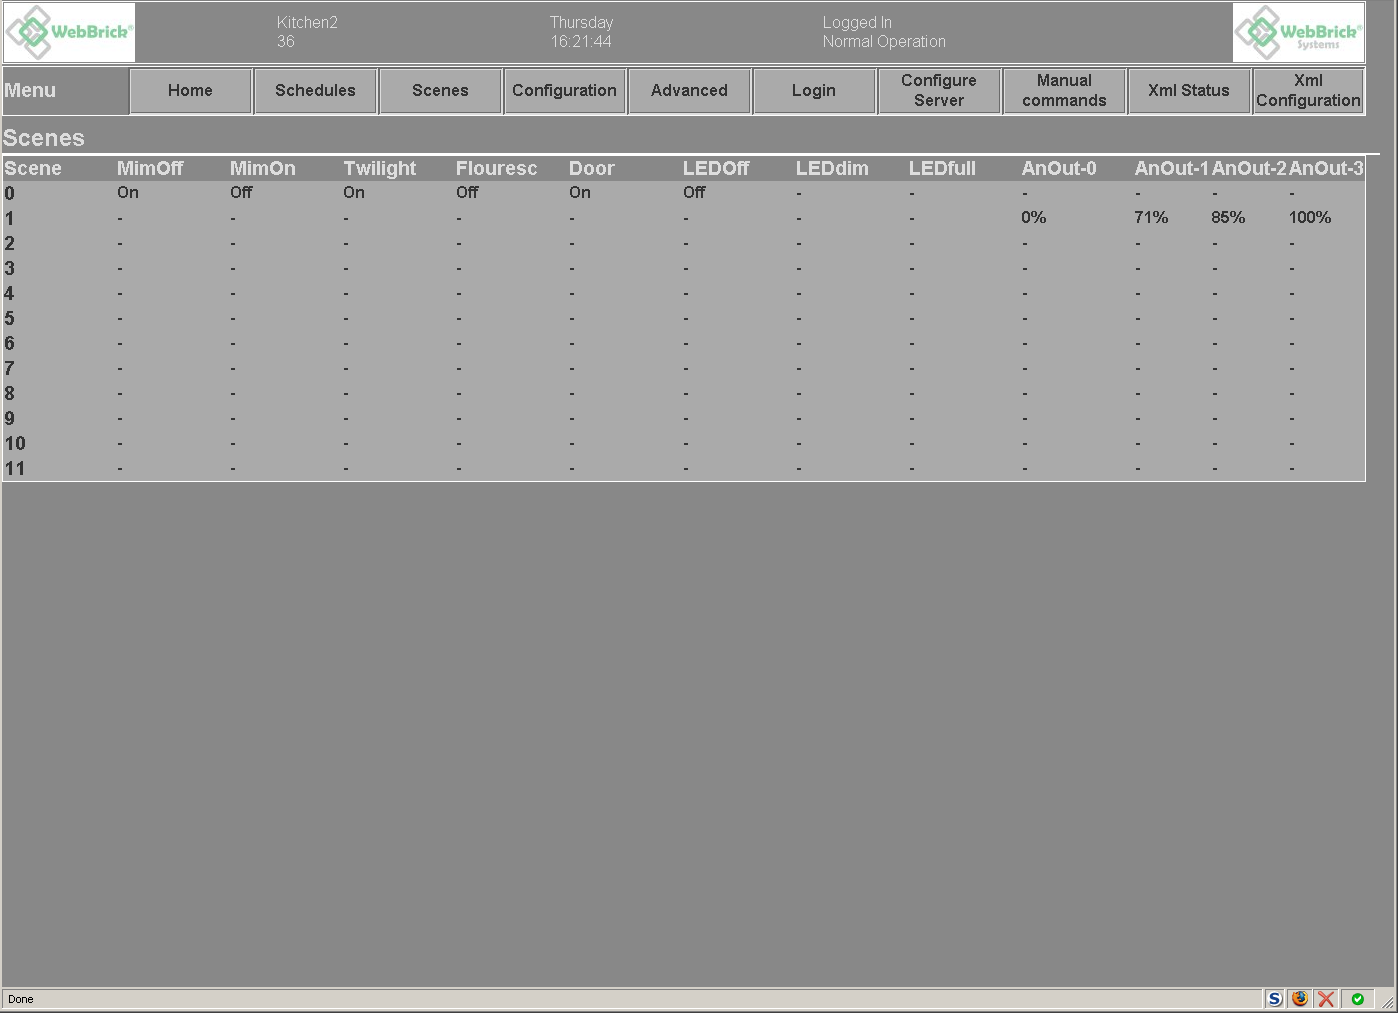
\includegraphics[width=0.8\textwidth]{Images/Scenes.png}
\caption{WebBrick Scenes Page}
\end{figure}

This page shows the current setting of configured scenes, if logged in you can click on an entry and reconfigure a scene.
A scene consists of an setting for each analogue and digital output channel, this setting may be ignore in which case 
no change is made to the relevant output channel. For digital channels
the options are:

	\begin{itemize}
		\item{\bf Ignore} Do nothing to this output when the scene is selected
		\item{\bf Off} Switch OFF this output when the scene is selected
		\item{\bf On} Switch ON this output when the scene is selected
	\end{itemize}

For analogue channels it is the any of the preset points or Ignore. 

If a scene is triggered by a local event this will have an action associated with it, this action is used on all digital
channels that are not Ignore or Off and for analogue channels that are not being Ignored. The result of this is that
you can perform any action on the scene such as Dwell to bring a scene on for a time period.

Note that from 6.3 onwards, scenes may be in two banks, 0-7 and 8-11.  This allows scenes to be used in two areas, for example
a major and minor room.

\begin{figure}[H]
\centering
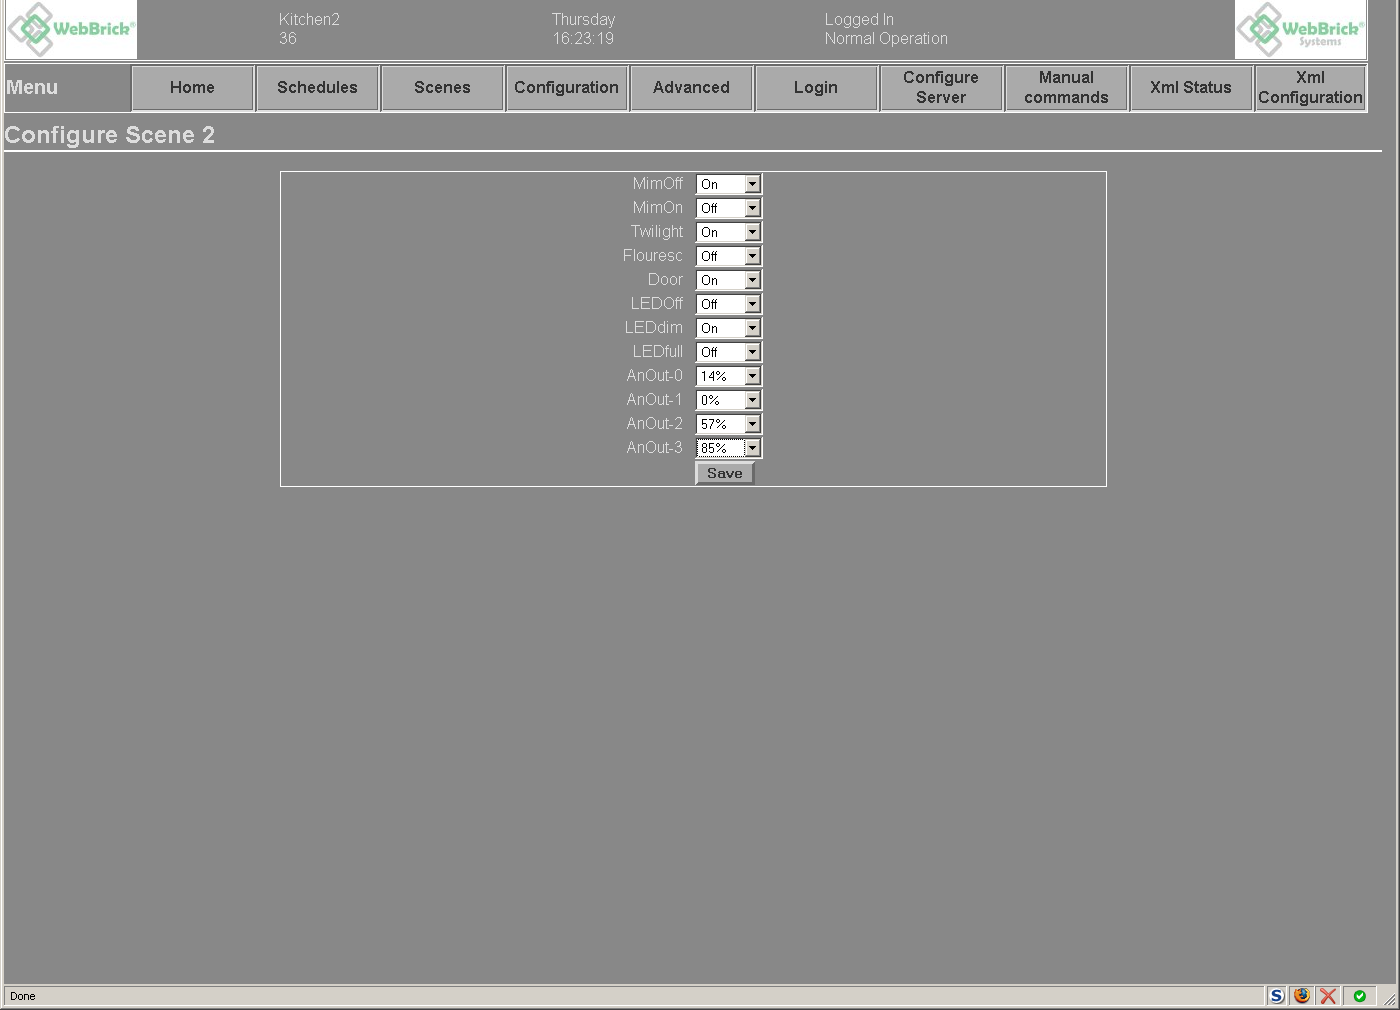
\includegraphics[width=0.8\textwidth]{Images/Scene.png}
\caption{WebBrick Scene configuration Page}
\end{figure}


\subsubsection{Scenes with Digital Inputs}
\index{Scenes - Configuration}

 At WebBrickSystems we've found that the following configuration gives a great deal of flexibility, usability when using scenes.
 
 Consider a 'major' and 'minor' room, or a through room with related areas, the organize the buttons thus:
 
	\begin{itemize}
		\item{\bf RoomMajOff} - {\em Action:ON Scene:0}
		\item{\bf RoomMajNext} - {\em Action:ON Scene:Last i.e. up to 7}
		\item{\bf RoomMinOff} - {\em Action:ON Scene:8}
		\item{\bf RoomMinNext} - {\em Action:ON Scene:11}
	\end{itemize}

 Now organise the scenes and Mimic outputs thus 

\begin{figure}[H]
\centering
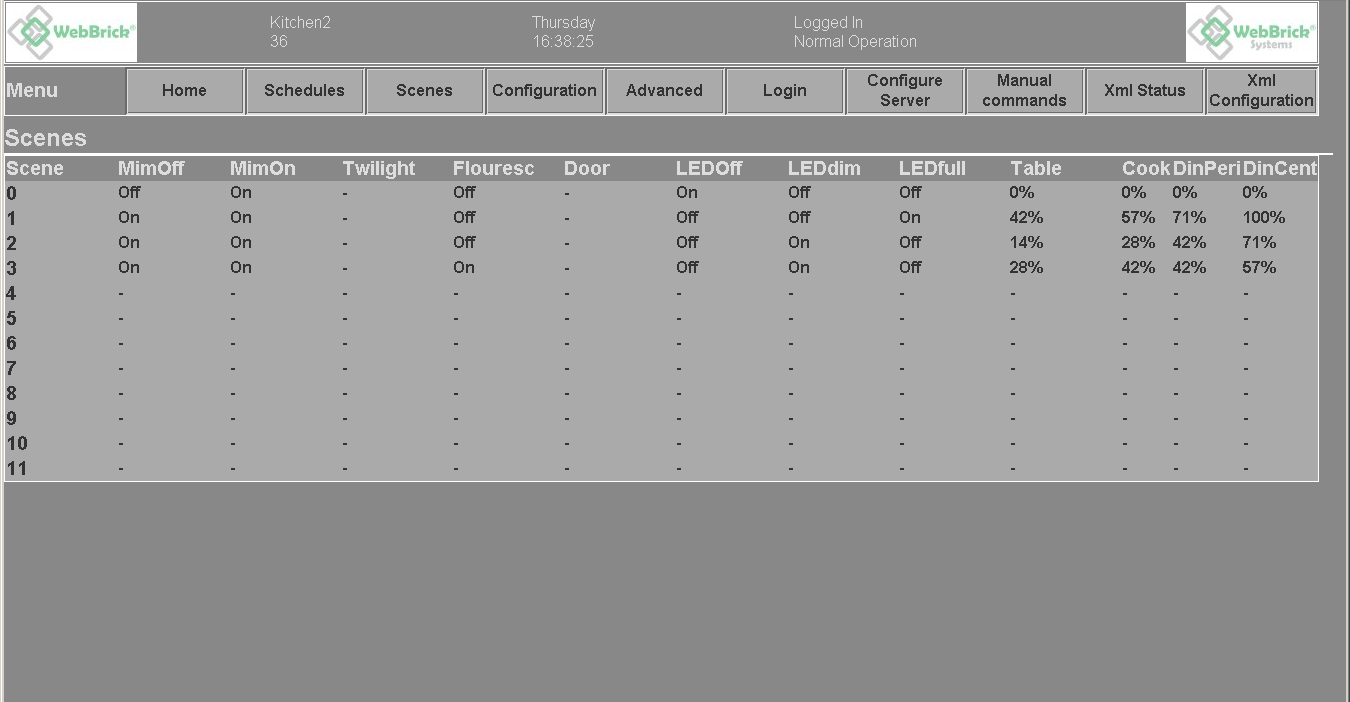
\includegraphics[width=0.8\textwidth]{Images/SceneMimics.png}
\caption{WebBrick Scene configuration Page}
\end{figure}

Note that the mimics help the user to see where they are in the sequence, thus

	\begin{itemize}
		\item{\bf Off Mimic - OFF, Next Mimic - ON} {\em Must be at the off, or begining of the sequence } 
		Only option is to press the 'Next' button, indicated because it is more bright. 
		\item{\bf Off Mimic - ON, Next Mimic - ON} {\em Must be somewhere mid sequence }
		Options 'Next' and 'Off' are valid.
		\item{\bf Off Mimic - ON, Next Mimic - OFF} {\em Must be at the off, or begining of the sequence }
		Only option is 'Off' since the end of the sequence has been reached.
	\end{itemize}



\subsection{Configuration}
From this page you can see the current settings of the various inputs and outputs, 
if logged in you can click to change the settings. You can change the names of inputs and 
outputs and change the trigger settings for the inputs. You can also change the length of the 
Dwells, adjust the analogue presets and alter the lower and upper threshold triggers for the temperature
sensors and analogue inputs.

\begin{figure}[H]
\centering
\includegraphics[width=0.8\textwidth]{Images/configuration.jpg}
\caption{WebBrick Configuration Home Page}
\end{figure}

\begin{tabular}{l|p{12cm}}
Section&Description\\
\hline
Digital Outputs&The first section shows the names of digital outputs. \\

Digital Inputs&The third section shows the configuration of the digital inputs. The Name column header can be
clicked to rename the channels and each row can be clicked to reconfigure the trigger.\\

Analogue Outputs&
The fourth section shows the Analogue outputs and by clicking the Name header the channels can be renamed.\\

Analogue Inputs&
The fifth section shows the Analogue inputs. By clicking the Name header the channels can be renamed and 
by clicking on an entry the high or low threshold triggers can be configured.\\

Temperature Inputs&
The sixth section shows the temperature inputs. By clicking tha Name header the channels can be renamed and 
by clicking on an entry the high or low threshold triggers can be configured.\\

Dwell Times&
The seventh section shows the value's for the dwell times formatted into seconds, minutes, hours etc.\\

Analogue presets&
The final section shows the value's for the analogue presets.\\
\end{tabular}

\subsection{Digital Inputs}

\begin{figure}[H]
\centering
\includegraphics[width=0.8\textwidth]{Images/digitalin.png}
\caption{WebBrick Digital In configuration page}
\end{figure}

The digital inputs can be configured to select the trigger target and whether to send a UDP packet. 
If you require no local action select action None from the action drop down box, 
if you do not require a UDP packet select none from the UDP type drop down box. 
A UDP Type of Remote is reserved for future enhancements.

\subsection{Naming channels}

\begin{figure}[H]
\centering
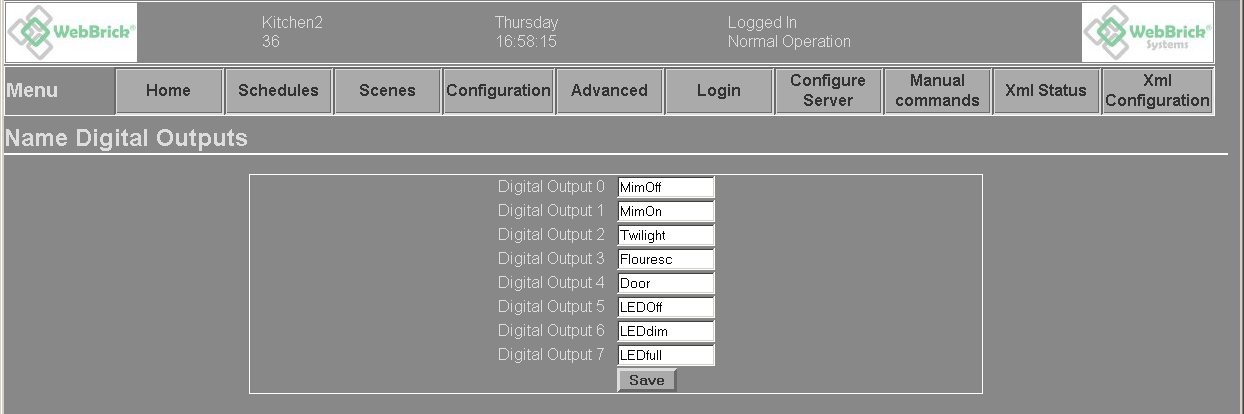
\includegraphics[width=0.8\textwidth]{Images/NameDigitalOut.png}
\caption{WebBrick Name digital outputs page}
\end{figure}

All input and output channels can be renamed to give them meaningful names for the use they are put to. 
Clicking on a Naming link will show a page similar to this where you can change the names for a whole group and then save it.

\subsection{Thresholds}

\begin{figure}[H]
\centering
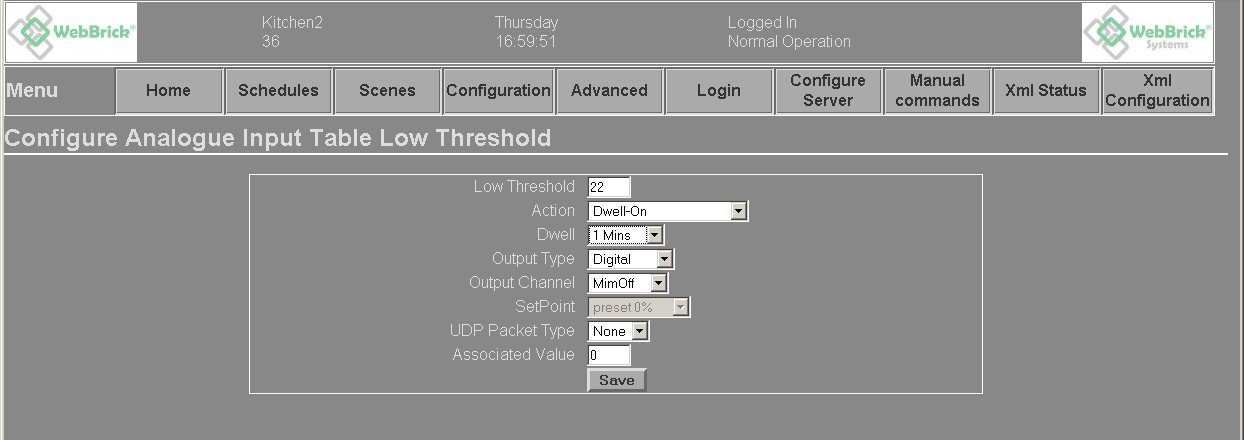
\includegraphics[width=0.8\textwidth]{Images/AnalogueThresh.png}
\caption{WebBrick Analogue threshold configuration page}
\end{figure}

The analogue inputs and temperature sensors can be configured with high and low thresholds, on selecting the entry from the main screen you will be presented with a form like this where you enter the threshold value and the trigger details.

\subsection{Advanced}

\begin{figure}[H]
\centering
\includegraphics[width=0.8\textwidth]{Images/advanced.png}
\caption{WebBrick Advanced Page}
\end{figure}

\index{Advanced}
The advanced page allows you to see the WebBrick software version and IP address it also lets you view the Status and configuration as XML. 
A manual command input menu entry is displayed which will prompt you to login if not currently logged in. 
The level 2 password can also be changed.

\subsection{XmlStatus}
\index{XMLStatus}
This is a link to the XML status page from the WebBrick. This is intended to be accessed by central controllers to get status detail.

\subsection{XmlConfiguration}
\index{XMLConfiguration}
This is the link to the XML page that describes the full configuration of the WebBrick.
This is intended to be accessed by central controllers to get configuration information.

\subsection{Manual Commands}
\index{Manual Commands}

Here you can use the command syntax described later in this document.
Please be careful with these commands.  The WebBrick has error checking, but you as a user may issue commands that cause unexpected operation.

\subsection{Configure Server}
\index{Configure Server}
The Configure server page lets you set the time, Node name and IP address and Rotary encoder step, analogue fade rate.
These are displayed as three separate groups, clicking Save only saves the group the Save button belongs to.

\begin{figure}[H]
\centering
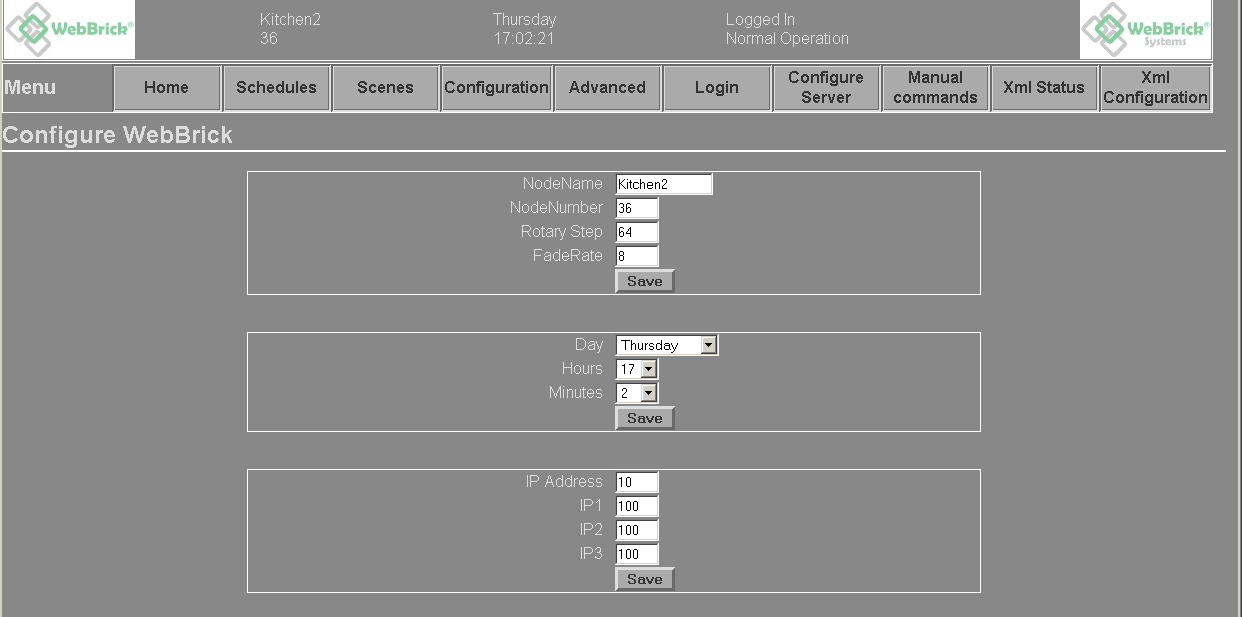
\includegraphics[width=0.8\textwidth]{Images/ConfigureServer.png}
\caption{WebBrick Configure Server Page}
\end{figure}


\subsection{Login}
\index{Login}
\begin{figure}[H]
\centering
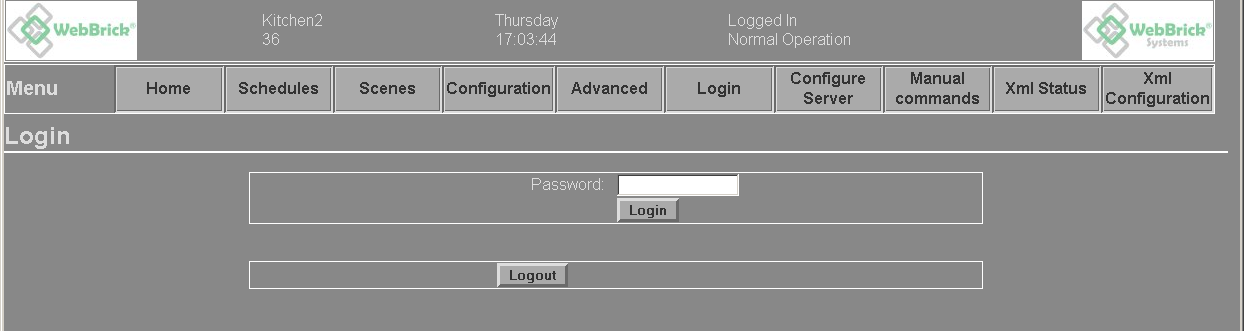
\includegraphics[width=0.8\textwidth]{Images/login.png}
\caption{WebBrick Login Page}
\end{figure}

The login page allows you to enter a password to enable changing the WebBrick configuration. The
login times out 5 minutes after the last command that changes the configuration. Attempts to make
changes when login has timed out will result in the command being ignored and an error condition displayed. 
The WebBrick has 3 passwords which give different levels of access. 

\begin{tabular}{l|p{12cm}}
Level&Description\\
\hline
1&password is normally blank and enables the control buttons on the home page.\\
2&password default is "password" and enables general reconfiguration.\\
3&password default is "installer" and enables reconfiguration.\\
\end{tabular}

To change a password you have to be logged in to at least the level the password applies to.
